\documentclass[12pt]{article}
\usepackage[margin=2.5cm]{geometry}
\usepackage{enumerate}
\usepackage{amsfonts}
\usepackage{amsmath}
\usepackage{fancyhdr}
\usepackage{amsmath}
\usepackage{amssymb}
\usepackage{amsthm}
\usepackage{mdframed}
\usepackage{graphicx}
\usepackage{subcaption}
\usepackage{adjustbox}
\usepackage{listings}
\usepackage{xcolor}
\usepackage{booktabs}
\usepackage[utf]{kotex}
\usepackage{hyperref}

\definecolor{codegreen}{rgb}{0,0.6,0}
\definecolor{codegray}{rgb}{0.5,0.5,0.5}
\definecolor{codepurple}{rgb}{0.58,0,0.82}
\definecolor{backcolour}{rgb}{0.95,0.95,0.92}

\lstdefinestyle{mystyle}{
    backgroundcolor=\color{backcolour},
    commentstyle=\color{codegreen},
    keywordstyle=\color{magenta},
    numberstyle=\tiny\color{codegray},
    stringstyle=\color{codepurple},
    basicstyle=\ttfamily\footnotesize,
    breakatwhitespace=false,
    breaklines=true,
    captionpos=b,
    keepspaces=true,
    numbers=left,
    numbersep=5pt,
    showspaces=false,
    showstringspaces=false,
    showtabs=false,
    tabsize=1
}

\lstset{style=mystyle}

\pagestyle{fancy}
\renewcommand{\headrulewidth}{0.4pt}
\lhead{CSC 373}
\rhead{Worksheet 4 Solution}

\begin{document}
\title{CSC373 Worksheet 4 Solution}
\maketitle

\bigskip

\begin{enumerate}[1.]
    \item

    \begin{itemize}
        \item Calculating out-degree

        \bigskip

        Let $G = (V,E)$ be a directed graph. Let $[v_1,...,v_n]$ be a list of vertices
        in graph $G$.

        \bigskip

        I need to calculate the outdegree of every vertex using adjacency list.

        \bigskip

        We know that in addition to counting each $v_i$ in adjacency list where $i = 1, .., n$,
        we are also counting $\lvert Adj[v_i] \rvert$ edges.

        \bigskip

        Since there are $\lvert V \rvert = n$ many vertices, we can write that
        the total count is $\lvert V \rvert + \sum\limits_{i=1}^{n} \lvert Adj[v_i] \rvert = \lvert V \rvert + \lvert E \rvert$,
        which is $\mathcal{O}(\lvert V \rvert + \lvert E \vert)$.

        \bigskip

        \item Calculating In-degree

        \bigskip

        The outdegree of a vertex is indegree of another vertex.

        \bigskip

        Using this fact, we can conclude the running time of computing indegree of every vertax is $\mathcal{O}(\lvert V \rvert + \lvert E \vert)$.

    \end{itemize}

    \underline{\textbf{Notes:}}

    \bigskip

    \begin{itemize}
        \item \textbf{Vertex}
        \begin{itemize}
            \item Is a fundamental unit of which graphs are formed
            \item Also means node

            \begin{center}
            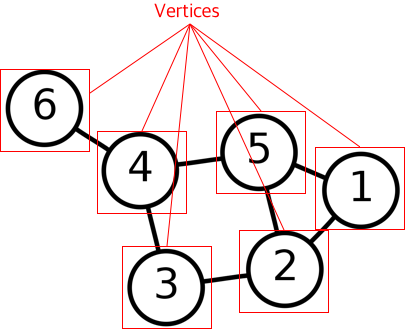
\includegraphics[width=0.4\linewidth]{images/worksheet_4_solution_1.png}
            \end{center}
        \end{itemize}

        \item \textbf{Adjacency-list Representation}
        \begin{itemize}
            \item Associates each vertax in a graph with the collection of its neighbouring vertices or edges
            \item Is represented by $Adj[v]$
            \begin{itemize}
                \item Means all vertices that are neighbour to vertex $v$
                \item In a directed graph, $Adj[v]$ are all out-degree vertices of vertax $v$
                \item $\lvert Adj[v] \rvert$ means the total number of outdegree of vertax $v$
            \end{itemize}
        \end{itemize}

        \begin{center}
        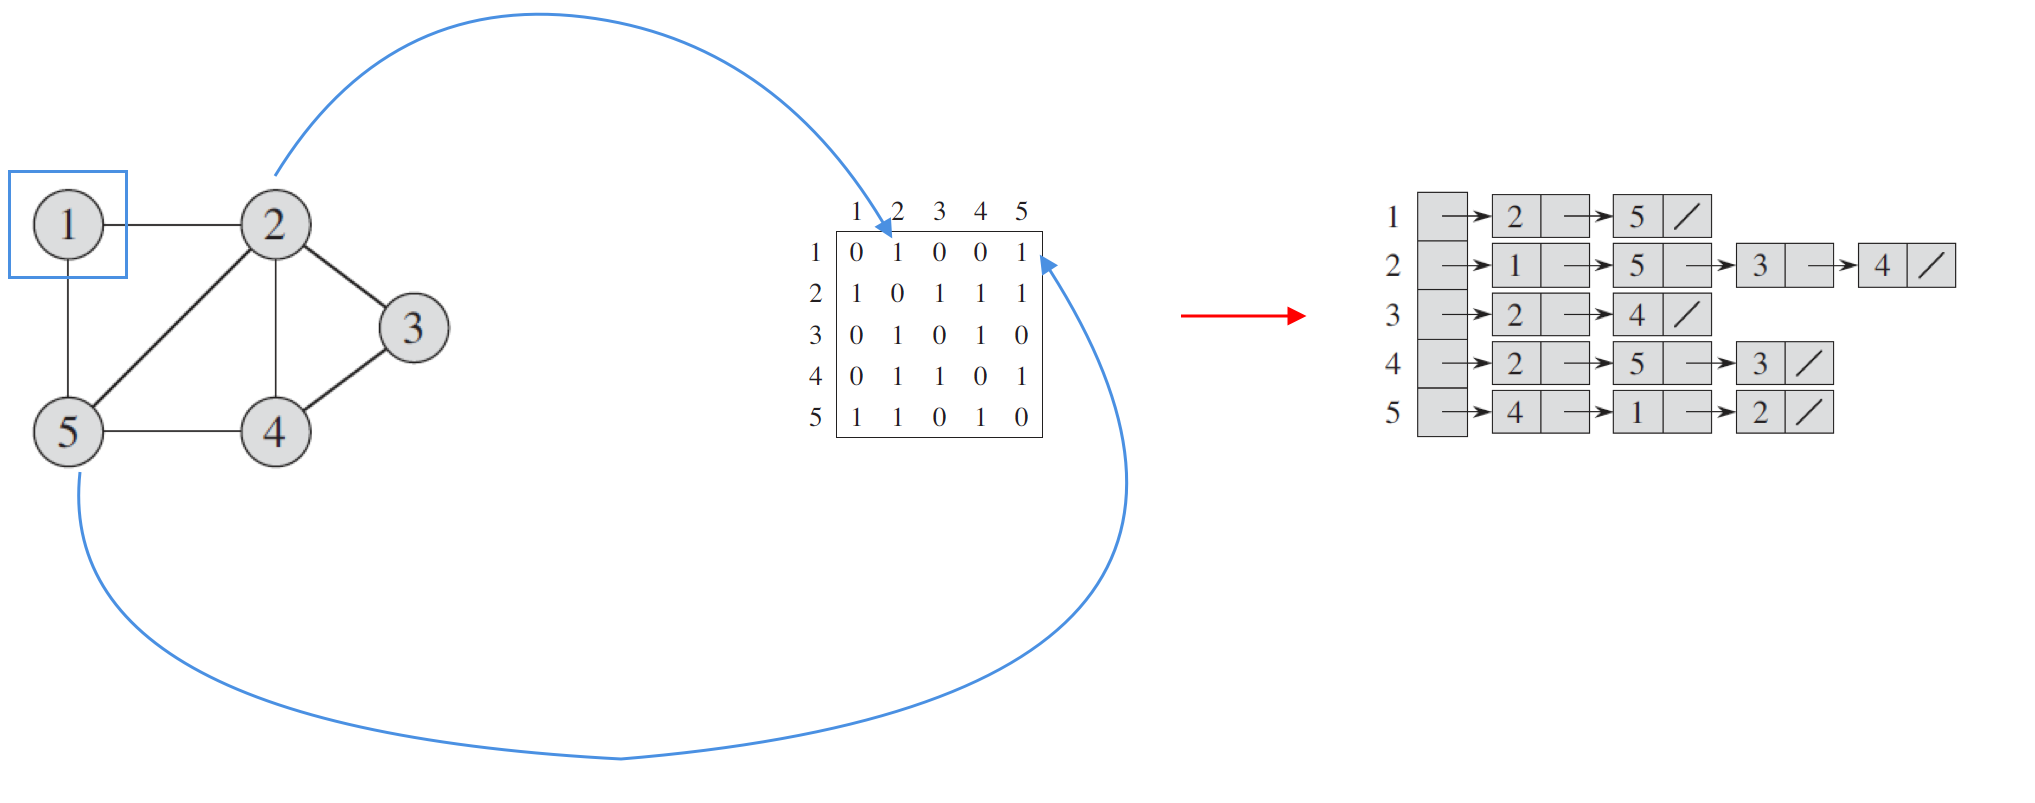
\includegraphics[width=\linewidth]{images/worksheet_4_solution_2.png}
        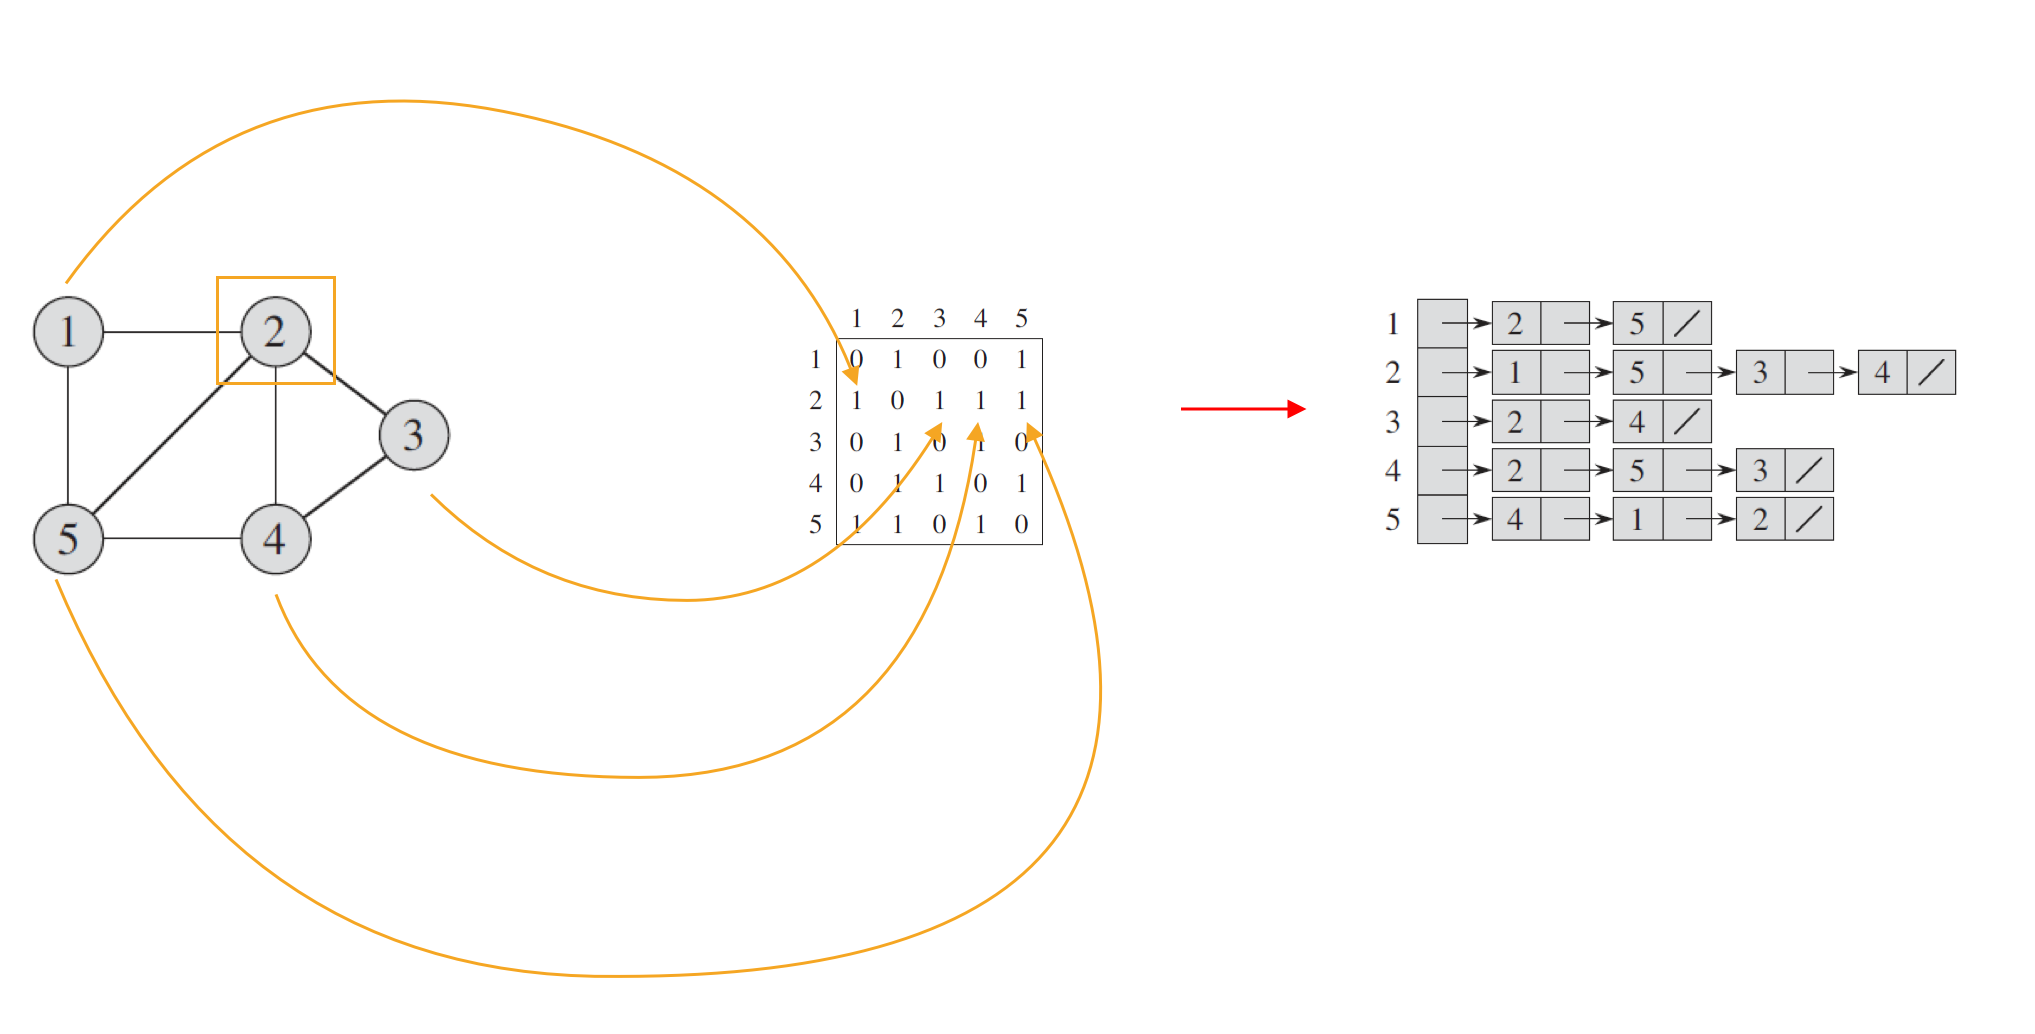
\includegraphics[width=\linewidth]{images/worksheet_4_solution_3.png}
        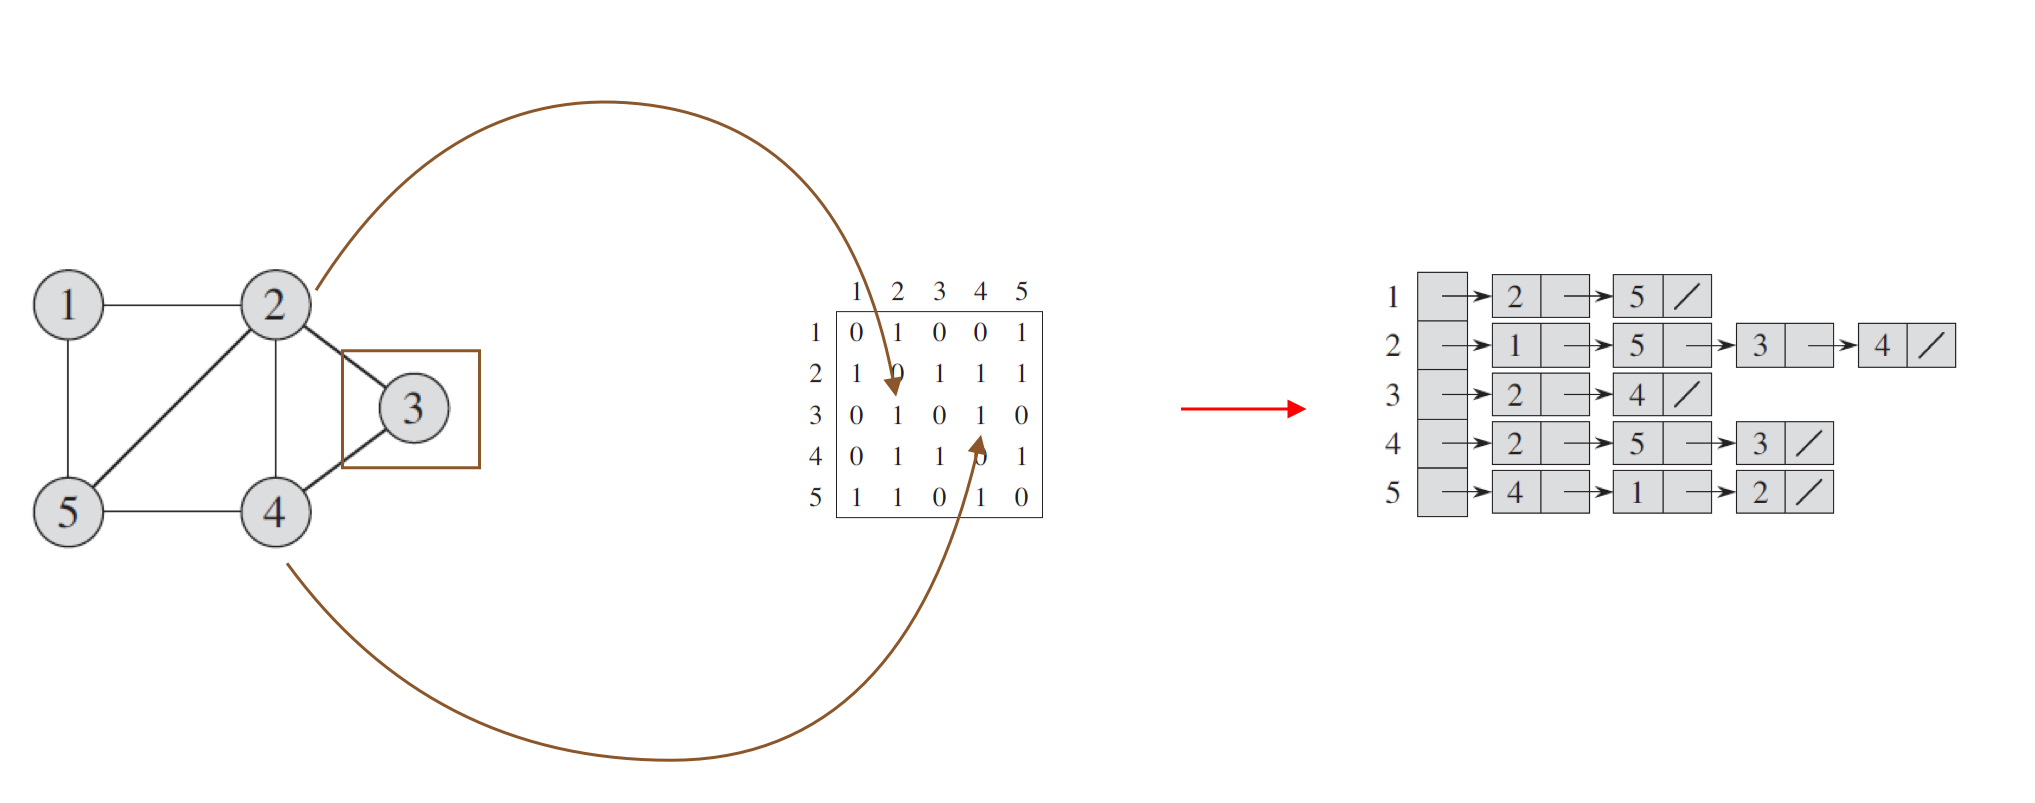
\includegraphics[width=\linewidth]{images/worksheet_4_solution_4.png}
        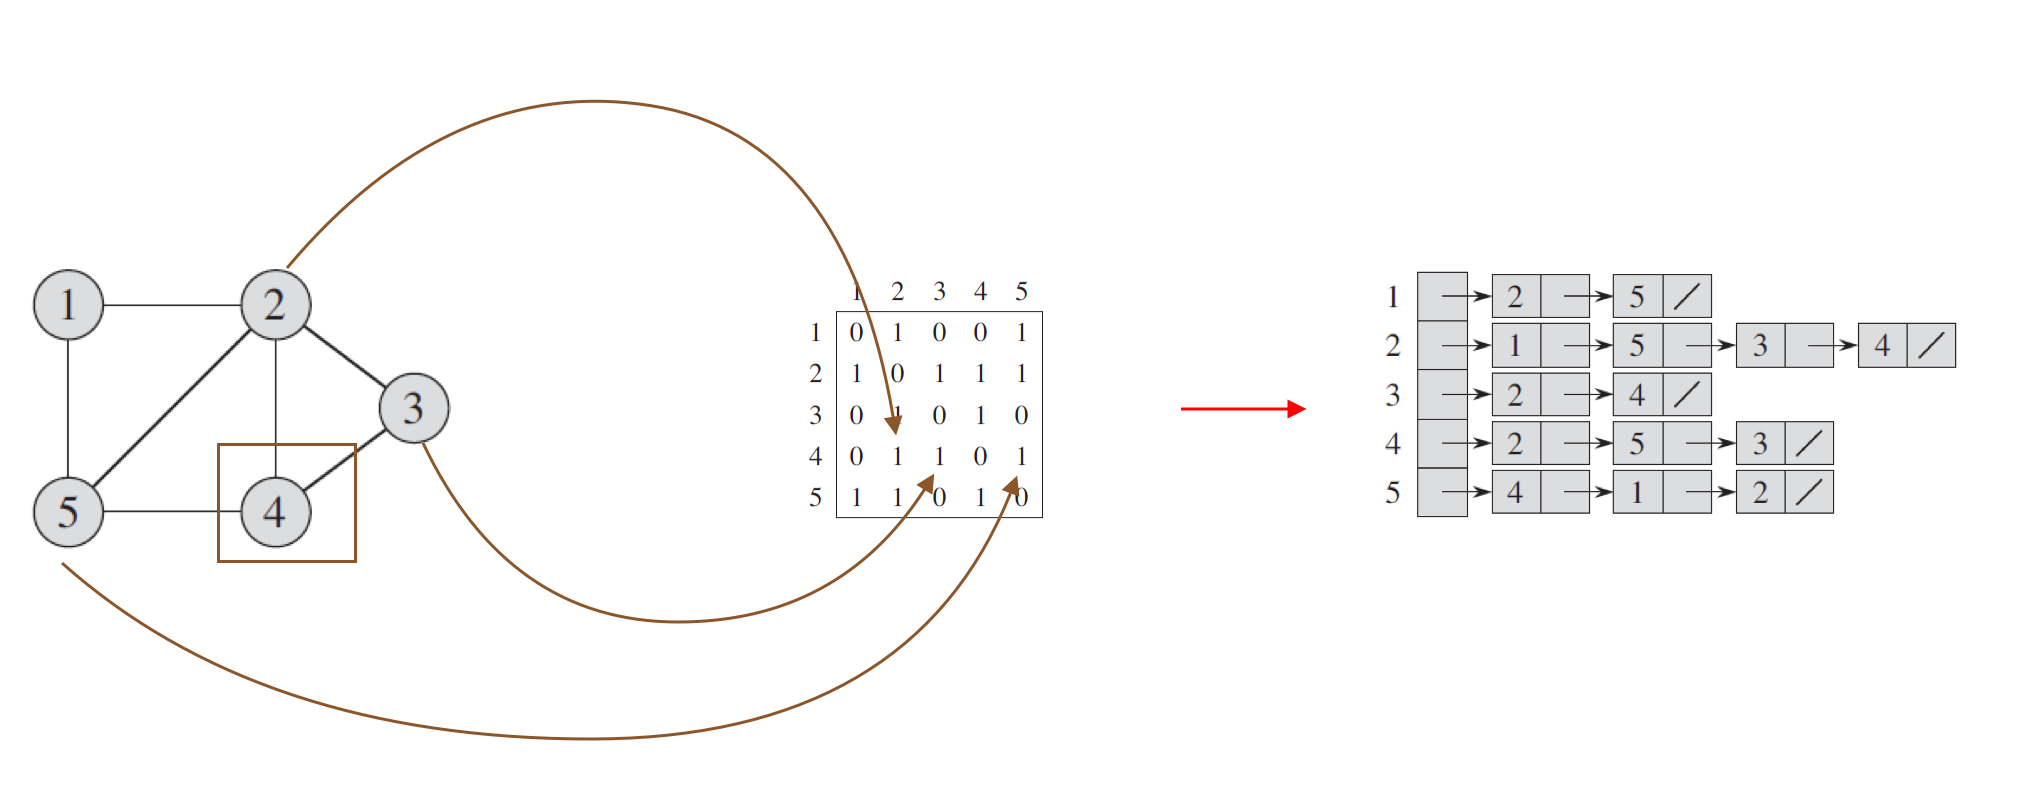
\includegraphics[width=\linewidth]{images/worksheet_4_solution_5.png}
        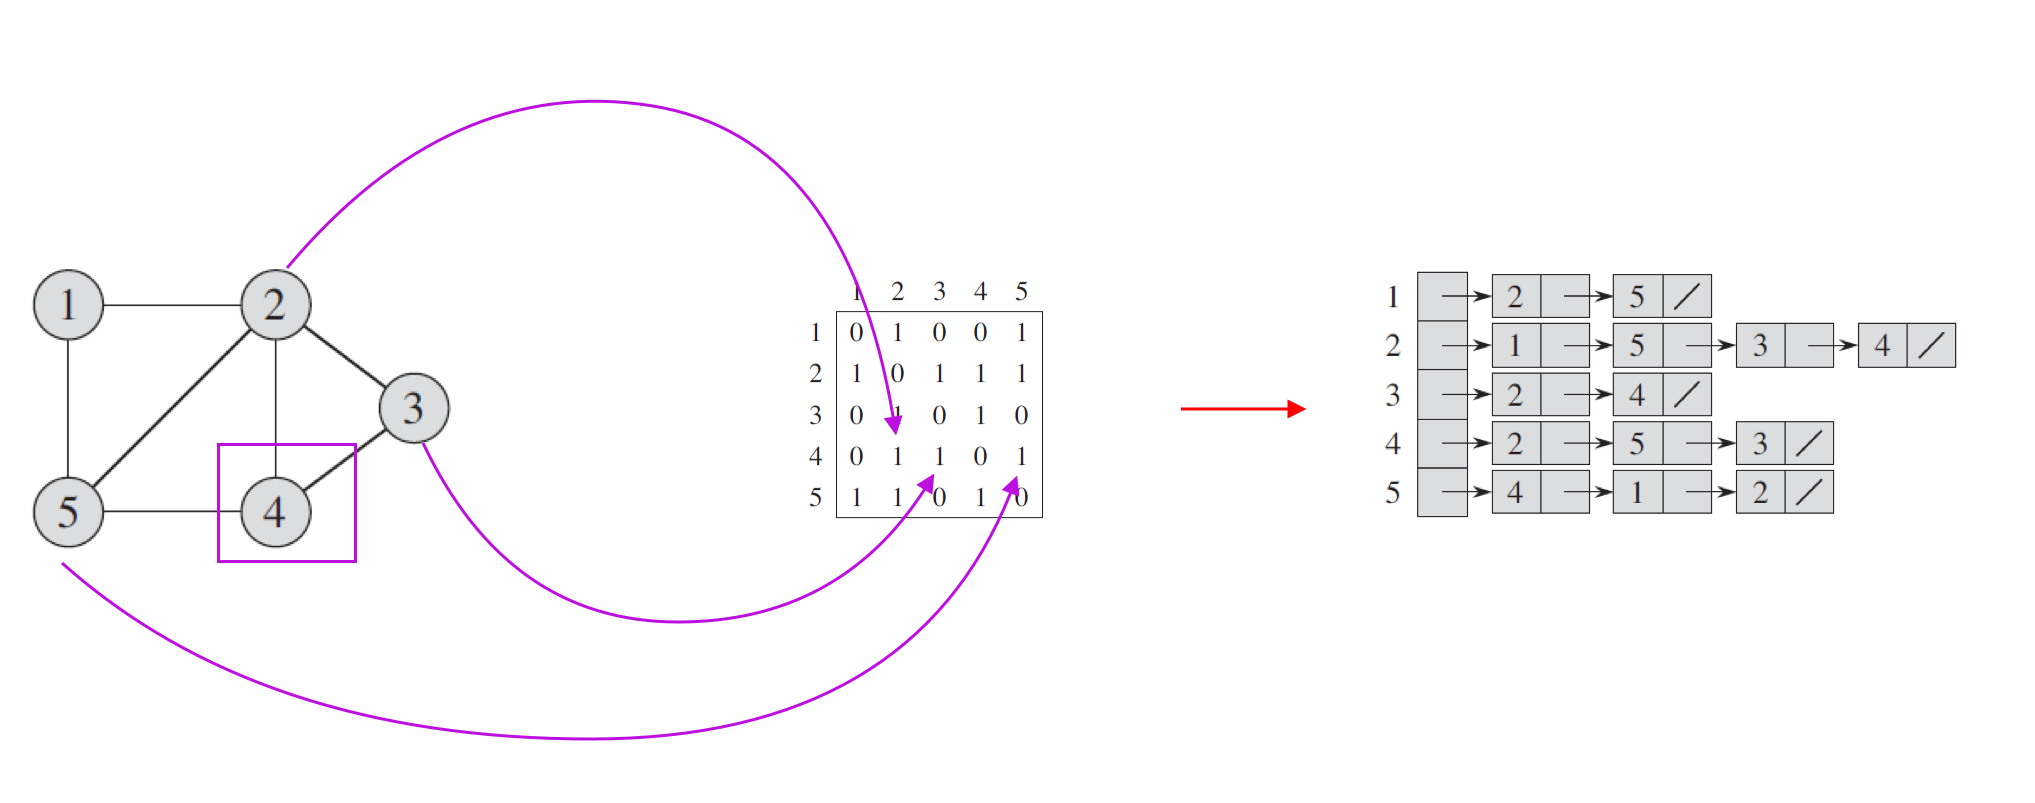
\includegraphics[width=\linewidth]{images/worksheet_4_solution_6.png}
        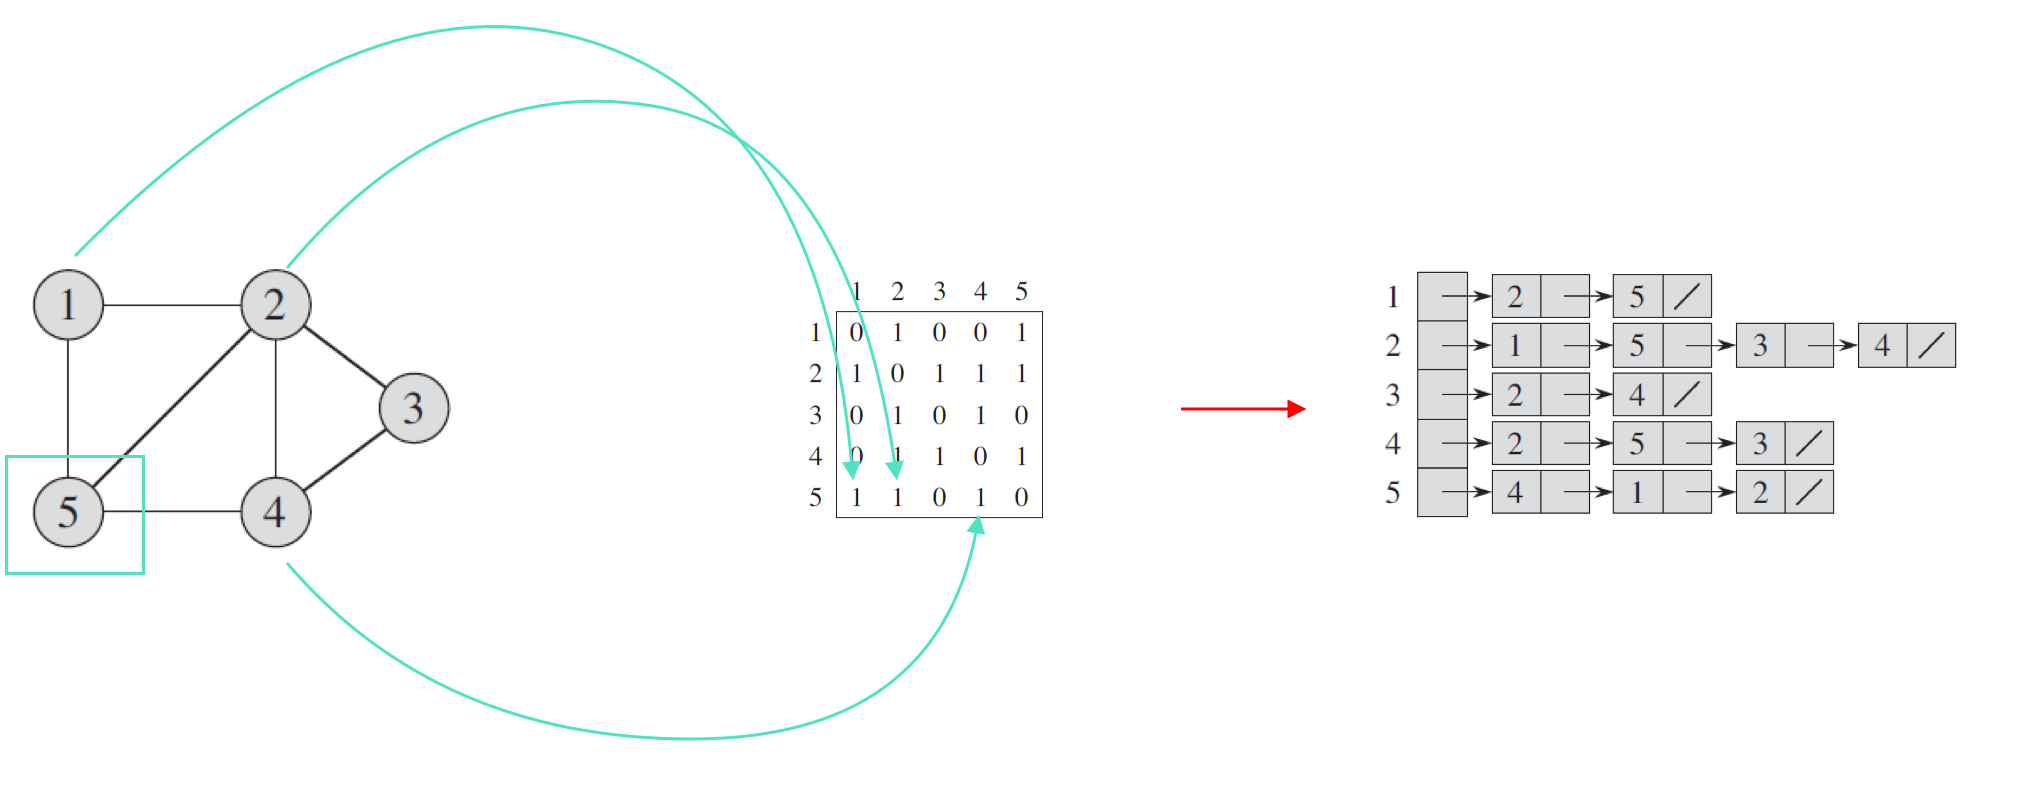
\includegraphics[width=\linewidth]{images/worksheet_4_solution_7.png}
        \end{center}

        \item \textbf{Directed graph}
        \begin{itemize}
            \item Is a graph that is made up of a set of vertices connected by edges,
            where the edges have a direction associated with them

            \begin{center}
            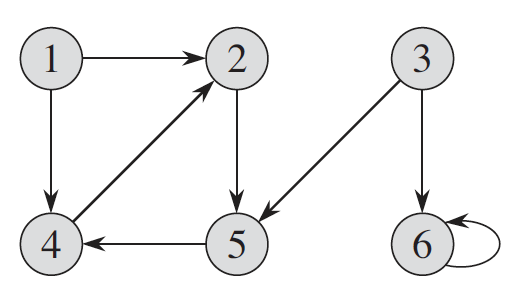
\includegraphics[width=0.4\linewidth]{images/worksheet_4_solution_8.png}
            \end{center}
        \end{itemize}

        \item \textbf{Out-degrees}
        \begin{itemize}
            \item For a directed graph $G=(V(G),E(G))$ and a vertex $x_1 \in V(G)$,
            the Out-Degree of $x_1$ refers to the number of arcs incident from $x_1$.
            That is, the number of arcs directed \underline{away} from the vertex $x_1$.

            \begin{center}
            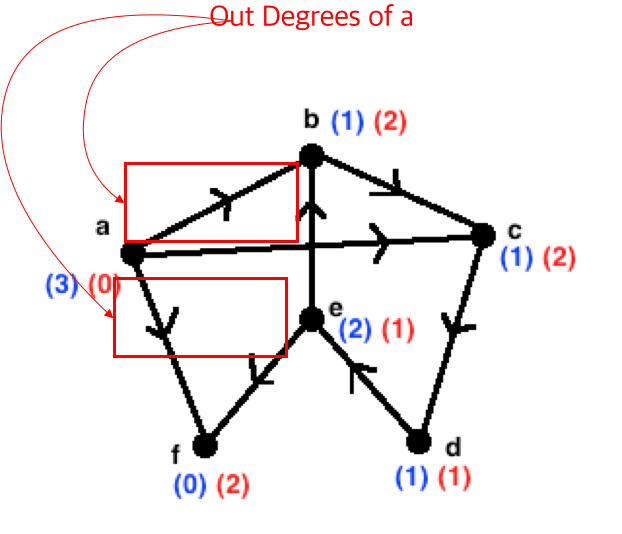
\includegraphics[width=0.4\linewidth]{images/worksheet_4_solution_9.png}
            \end{center}
        \end{itemize}

        \item \textbf{In-degrees}
        \begin{itemize}
            \item For a directed graph $G=(V(G),E(G))$ and a vertex $x_1 \in V(G)$,
            the In-Degree of $x_1$ refers to the number of arcs incident to $x_1$.
            That is, the number of arcs directed \underline{towards} the vertex $x_1$.

            \begin{center}
            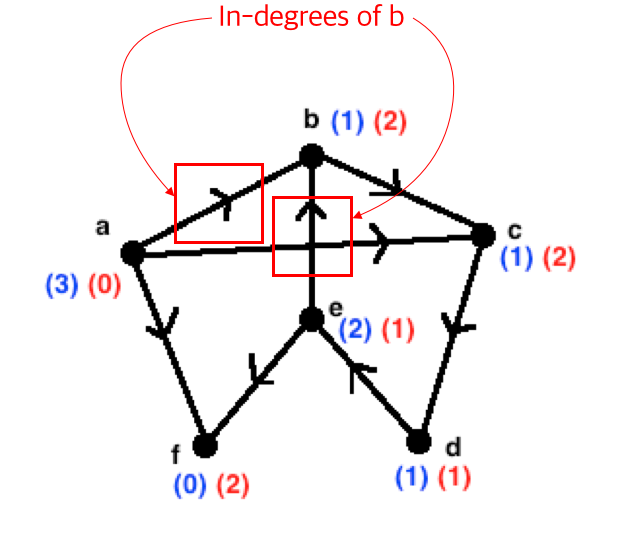
\includegraphics[width=0.4\linewidth]{images/worksheet_4_solution_10.png}
            \end{center}
        \end{itemize}

        \item Computing the outdegree of every vertex using adjacency list

        \bigskip

        \begin{center}
        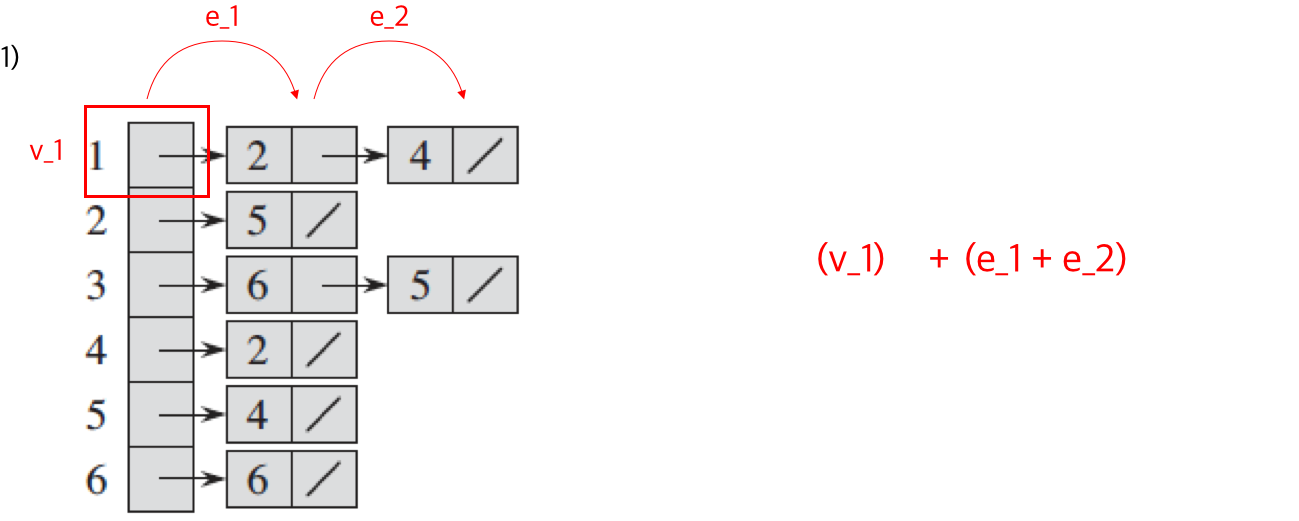
\includegraphics[width=\linewidth]{images/worksheet_4_solution_11.png}
        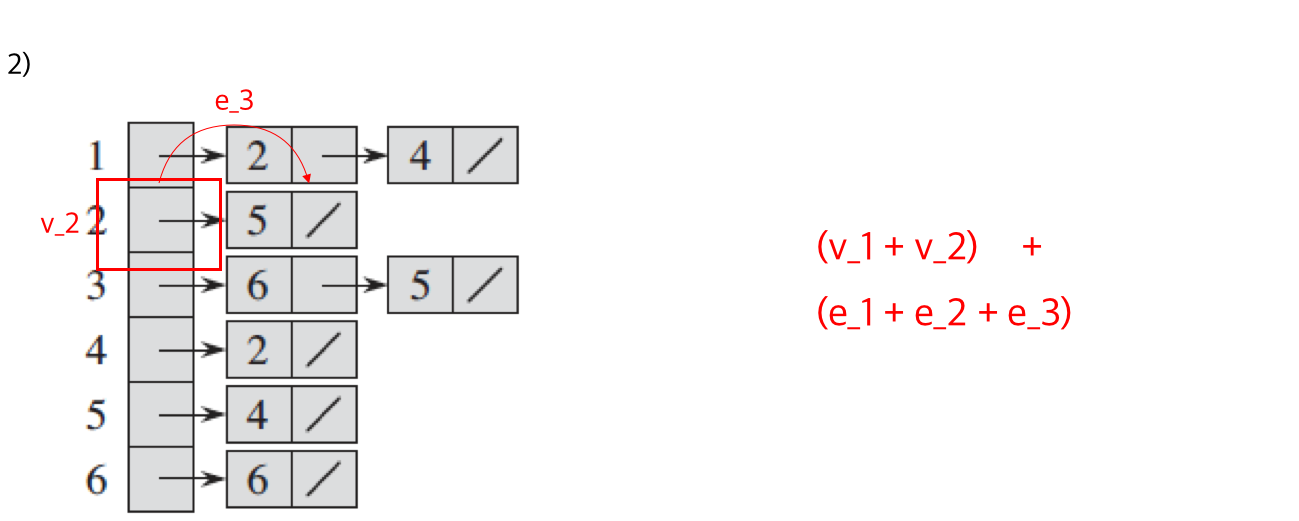
\includegraphics[width=\linewidth]{images/worksheet_4_solution_12.png}
        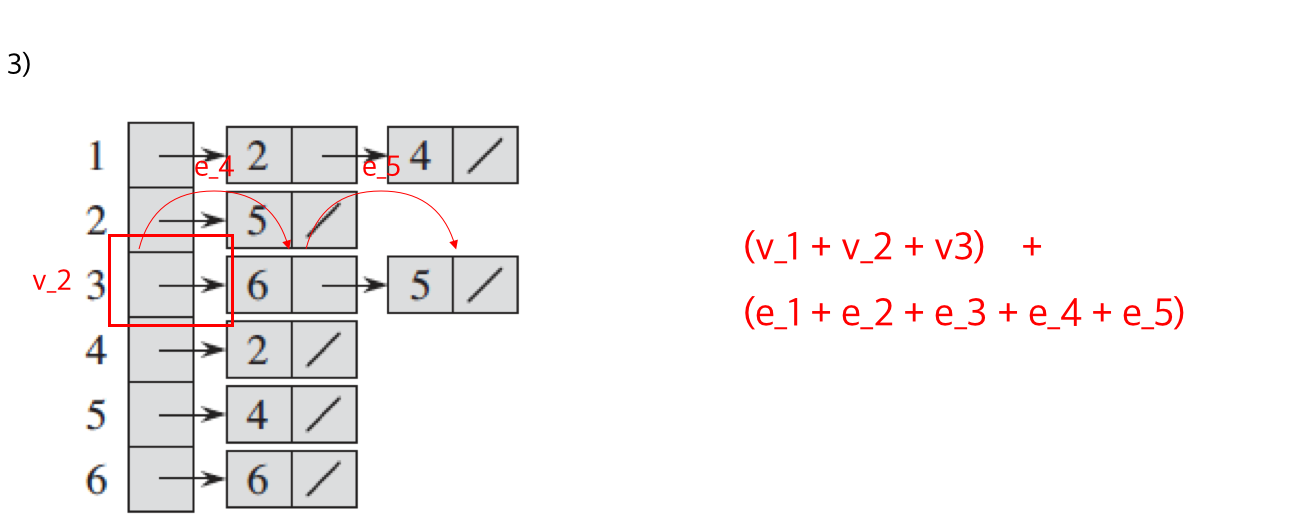
\includegraphics[width=\linewidth]{images/worksheet_4_solution_13.png}
        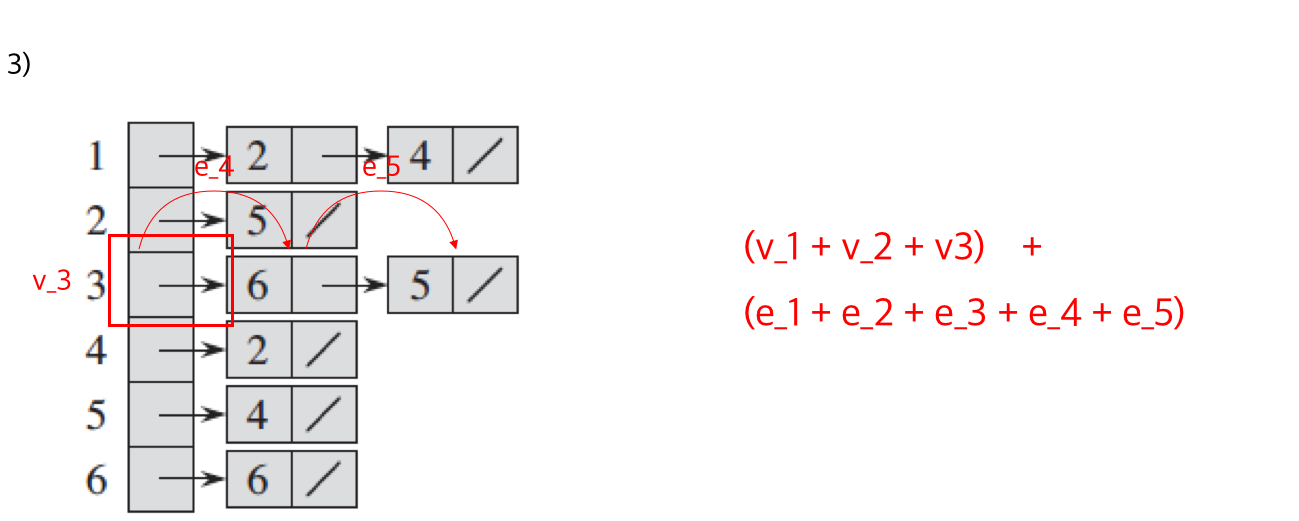
\includegraphics[width=\linewidth]{images/worksheet_4_solution_14.png}
        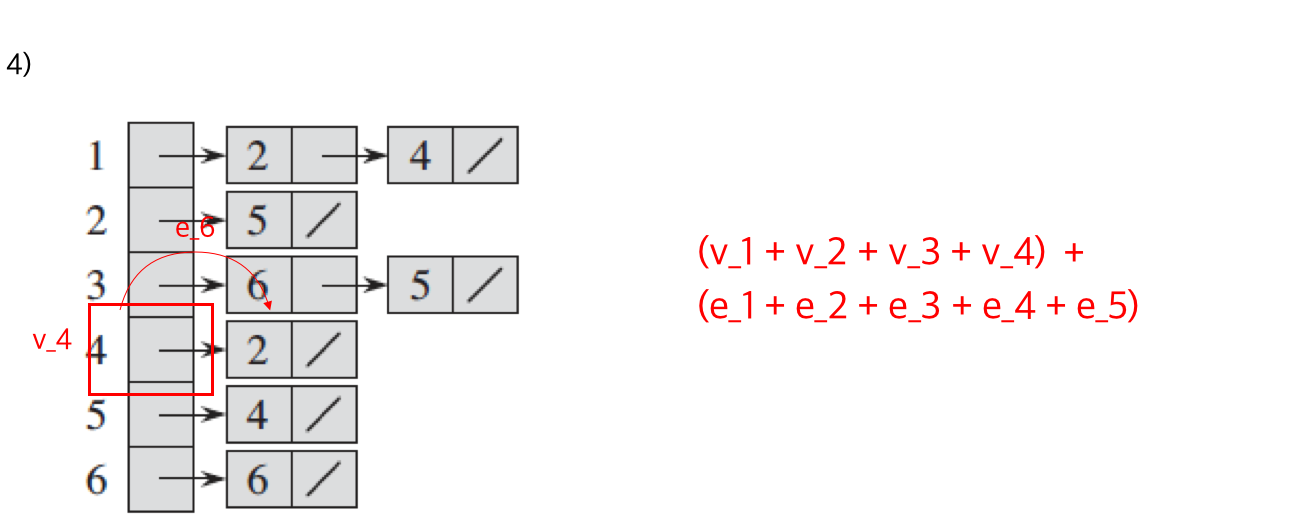
\includegraphics[width=\linewidth]{images/worksheet_4_solution_15.png}
        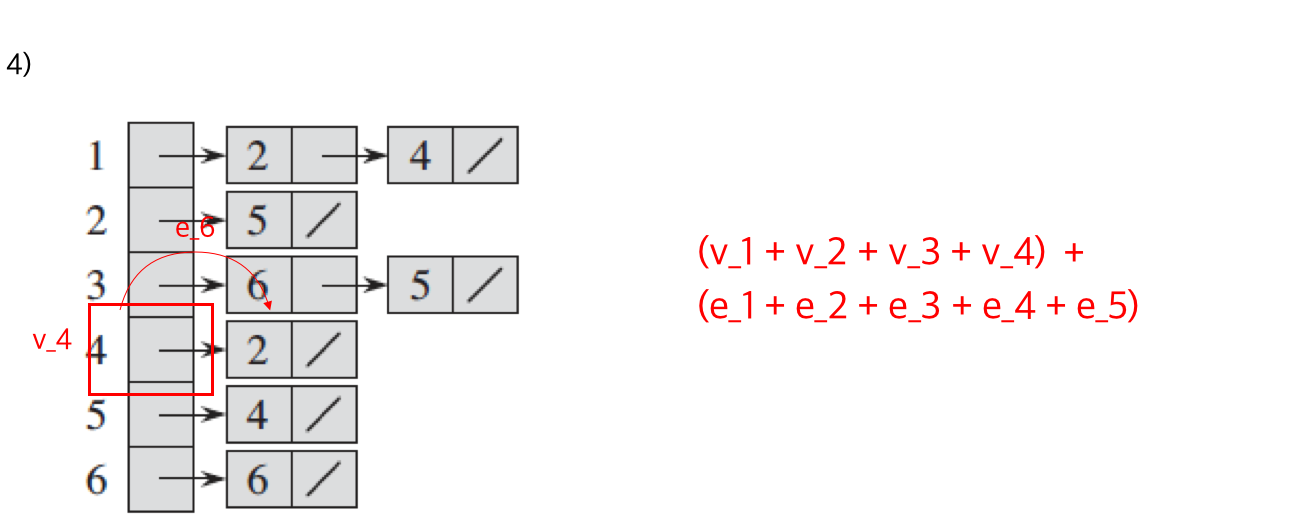
\includegraphics[width=\linewidth]{images/worksheet_4_solution_16.png}
        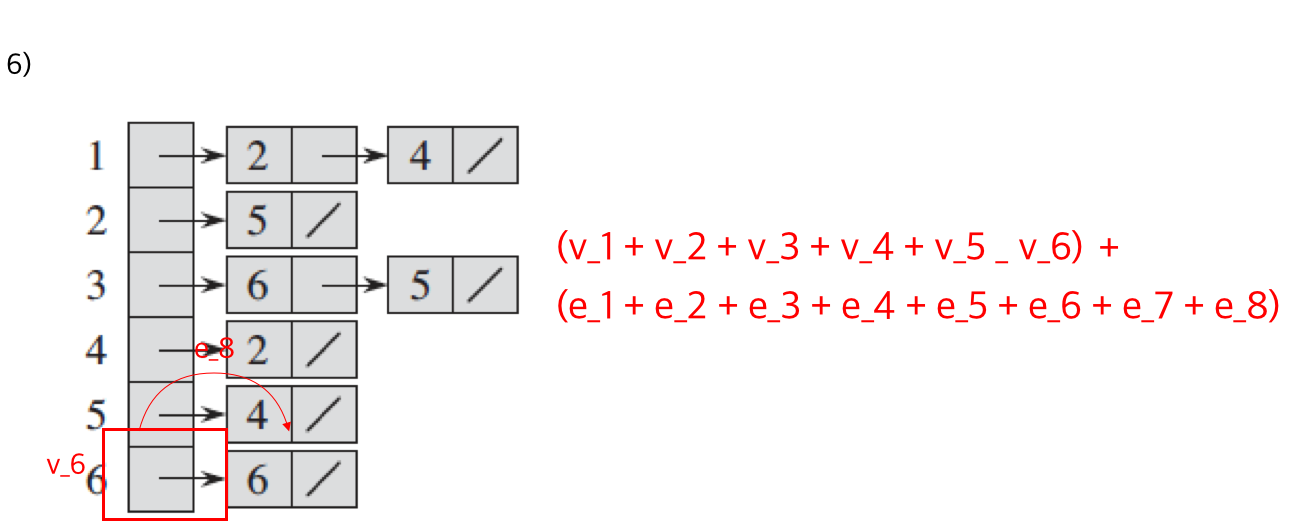
\includegraphics[width=\linewidth]{images/worksheet_4_solution_17.png}
        \end{center}

        \bigskip

        So it has $\mathcal{O}(V + E)$

        \item Computing the outdegree of every vertex using adjacency list

        \bigskip

        The outdegree of a vertex is indegree of another vertex.

        \bigskip

        Using this fact, we can conclude the running time of computing indegree of every vertax is $\mathcal{O}(V + E)$.
    \end{itemize}

    \item

    \begin{itemize}
        \item Computing $G^T$ from $G$ in Adjacency List

        \begin{center}
        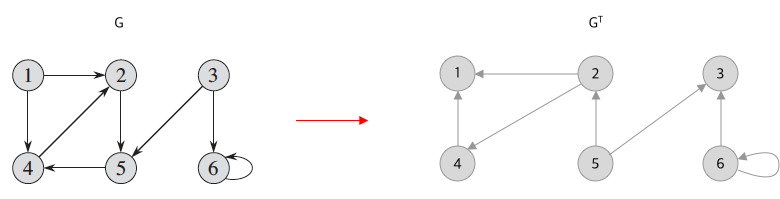
\includegraphics[width=\linewidth]{images/worksheet_4_solution_18.png}
        \end{center}

    \begin{lstlisting}[mathescape=true]
    COMPUTE-G-TRANSPOSE-ADJ-MATRIX(Adj,V)
        Let Adj' be a new adjacency list containing keys $v_i...v_n$

        for i = 1 to $\lvert V \rvert$
            for every vertax $w$ in Adj[$v_i$]
                Insert(Adj'[w], $v_i$)

        return Adj'
    \end{lstlisting}

        \item Computing $G^T$ from $G$ in Adjacency-Matrix

        \begin{center}
        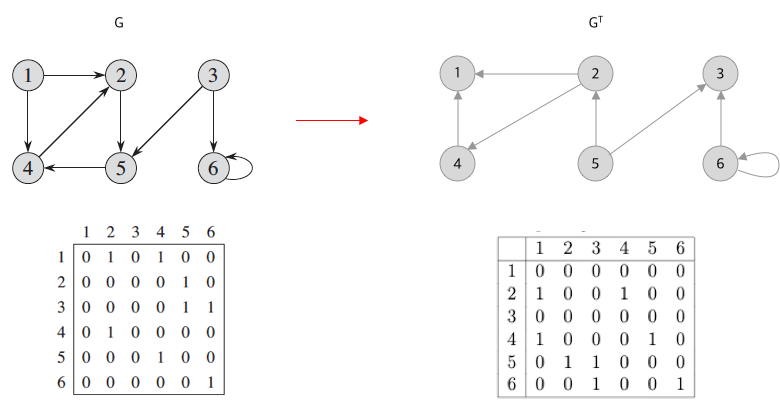
\includegraphics[width=\linewidth]{images/worksheet_4_solution_19.png}
        \end{center}

    \begin{lstlisting}[mathescape=true]
    COMPUTE-G-TRANSPOSE-ADJ-MATRIX(A,V)
        Let A'[1..$\lvert V \rvert$, 1..$\lvert V \rvert$] be a new adjacency matrix

        for i = 1 to $\lvert V \rvert$
            for j = 1 to $\lvert V \rvert$
                A'[j,i] = A[i,j]

        return A'
    \end{lstlisting}

    \bigskip

    \end{itemize}

    \bigskip


    \begin{mdframed}
        \underline{\textbf{Correct Solution:}}

        \bigskip

        \begin{itemize}
            \item Computing $G^T$ from $G$ in Adjacency List

            \begin{center}
            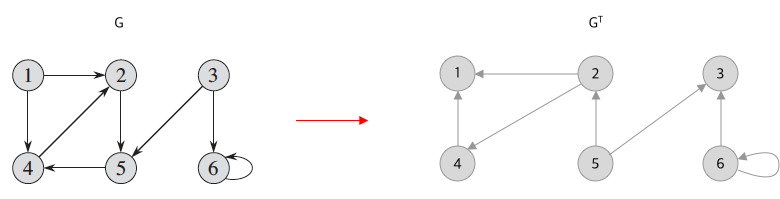
\includegraphics[width=\linewidth]{images/worksheet_4_solution_18.png}
            \end{center}

        \begin{lstlisting}[mathescape=true]
        COMPUTE-G-TRANSPOSE-ADJ-MATRIX(Adj,V)
            Let Adj' be a new adjacency list containing keys $v_i...v_n$

            for i = 1 to $\lvert V \rvert$
                for every vertax $w$ in Adj[$v_i$]
                    Insert(Adj'[w], $v_i$)

            return Adj'
        \end{lstlisting}

            \bigskip

            \color{red}The running time is $\mathcal{O}(\lvert V \rvert + \lvert E \rvert)$\color{black}

            \item Computing $G^T$ from $G$ in Adjacency-Matrix

            \begin{center}
            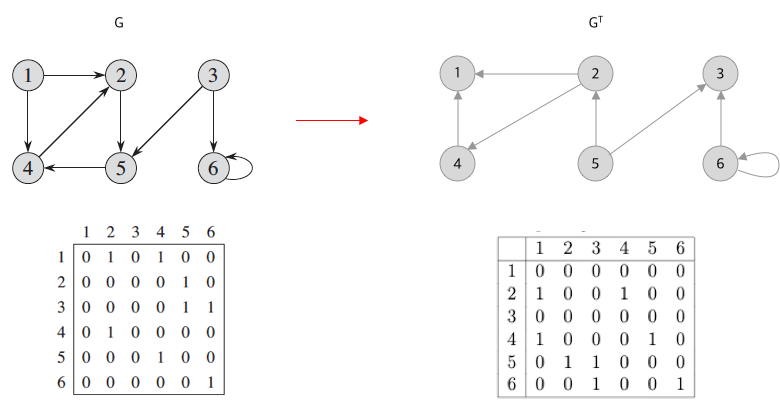
\includegraphics[width=\linewidth]{images/worksheet_4_solution_19.png}
            \end{center}

        \begin{lstlisting}[mathescape=true]
        COMPUTE-G-TRANSPOSE-ADJ-MATRIX(A,V)
            Let A'[1..$\lvert V \rvert$, 1..$\lvert V \rvert$] be a new adjacency matrix

            for i = 1 to $\lvert V \rvert$
                for j = 1 to $\lvert V \rvert$
                    A'[j,i] = A[i,j]

            return A'
        \end{lstlisting}

        \bigskip

        \color{red}The running time is $\mathcal{O}(\lvert V \rvert^2)$\color{black}


        \end{itemize}
    \end{mdframed}


    \item

    \bigskip

    \begin{lstlisting}[mathescape=true]
    Breadth-First-Search(V,$v_i$)
        d = 0
        for each $v_i \in V$
            while performing BFS(V, $v_i$)
                let $w$ be the current node in BFS
                    if $\delta($v_i$,w) > d$
                        d = $\delta(v_i, w)$

        return d
    \end{lstlisting}

    \bigskip

    \underline{\textbf{Notes:}}

    \bigskip

    \begin{itemize}
        \item \textbf{Breadth First Search}

        \begin{itemize}
            \item Is an algorithm for searching or traversing a graph
            \item Is one of the simplest algorithm
        \end{itemize}

        \item \textbf{Largest of All Shortest Path Distance}

        \bigskip

        \begin{itemize}
            \item Means the shortest distance between two furthest apart nodes

            \bigskip

            \begin{center}
            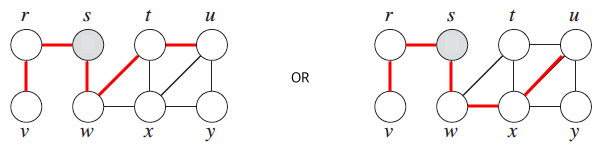
\includegraphics[width=\linewidth]{images/worksheet_4_solution_20.png}
            \end{center}
        \end{itemize}
    \end{itemize}


\end{enumerate}

\end{document}